\documentclass[12pt]{article}
\usepackage[hmargin={1in},vmargin={1in,1in},foot={.6in}]{geometry}   
\geometry{letterpaper}              
%\usepackage[parfill]{parskip}
\usepackage{color,graphicx}
\usepackage{setspace}
\usepackage{amsmath}
\usepackage{amssymb}
\usepackage{varioref}
\usepackage{textcomp}
%\usepackage{avm}
\usepackage{textcomp}
\usepackage{mflogo}
\usepackage{wasysym}
\usepackage[normalem]{ulem}
\usepackage{hyperref}
\usepackage{booktabs}

\newcommand{\HRule}{\rule{\linewidth}{0.25mm}}

\usepackage{fancyhdr} % This should be set AFTER setting up the page geometry
\pagestyle{plain} % options: empty , plain , fancy
\lhead{}\chead{}\rhead{}
\renewcommand{\headrulewidth}{.5pt}
\lfoot{}\cfoot{\thepage}\rfoot{}
\newcommand{\txtp}{\textipa}
\renewcommand{\rm}{\textrm}
\newcommand{\sem}[1]{\mbox{$[\![$#1$]\!]$}}
\newcommand{\lam}{$\lambda$}
\newcommand{\lan}{$\langle$}
\newcommand{\ran}{$\rangle$}
\newcommand{\type}[1]{\ensuremath{\left \langle #1 \right \rangle }}

\newcommand{\bex}{\begin{exe}}
\newcommand{\eex}{\end{exe}}
\newcommand{\bit}{\begin{itemize}}
\newcommand{\eit}{\end{itemize}}
\newcommand{\ben}{\begin{enumerate}}
\newcommand{\een}{\end{enumerate}}

%\linespread{1.5}
\thispagestyle{plain}

\title{Supporting information:\\ An excursus on noun effects}
\author{Gregory Scontras, Judith Degen, Noah D.~Goodman}
\date{}

\begin{document}

\maketitle

%Here we follow up on the finding that ordering preferences are not sensitive to noun-specific information in our original materials. 
Compositional (i.e., semantic) accounts of ordering preferences hold that the fundamental factor in predicting adjective ordering is whether or not an adjective is used to form a complex concept/subkind description: first you form the concept, then you modify it with additional adjectives (McNally and Boleda, 2004; Svenonius, 2008).\footnote{Bouchard 2005 makes a similar claim, namely that the formation of complex concepts can override adjective ordering preferences.} 
We find this hypothesis intriguing---perhaps concept-formability indeed determines ordering preferences (and therefore correlates with subjectivity).
%We considered it unlikely that a binary distinction like concept formation would be able to predict the gradience in our preference data. Still, we found the hypothesis very compelling, which is why 
As with our original experiments, the work in testing this hypothesis lies in operationalizing an abstract notion like whether or not an adjective tends to form a complex concept. 

%The literature on the topic  presupposes that intuitions about concept formability are systematic and generalizable, suggesting that they should be amenable to empirical investigation.
%
%\section{Experiment 1: Investigating concept-formability}
%
%According to McNally and Boleda, the key issue in diagnosing the formation of complex concepts is one of entailment. When an adjective modifies a noun intersectively, the objects described hold both the property named by the noun and the property named by the adjective: a ``male architect'' is both male and an architect (McNally and Boleda, 2004:179, ex.~2). When an adjective and a noun combine to form a complex concept (i.e., a subkind description), the objects described hold the property named by the noun, but not necessarily the property named by the adjective; the modification is (ostensibly) subsective. The authors give the Catalan example \emph{arquitecte t\`{e}cnic} ``technical architect,'' which names architects but not necessarily technical things (McNally and Boleda, 2004:179, ex.~1; cf.~the discussion of \emph{wild rice} in Svenonius 2008). 
%
%The semantic analysis given by these authors to adjectives that form complex concepts requires them to compose first with nouns, before run-of-the-mill intersective adjectives; thus, the fundamental factor in predicting adjective ordering ought to be whether an adjective forms a complex concept. The question thus becomes: does concept-formability predict ordering preferences? To answer this question, we tested whether the objects named by the adjective-noun descriptions in our original materials hold 1) the property named by the adjective, and 2) the property named by the noun. We then compared these data to the ordering preferences we measured in our naturalness rating experiment.
%
%\section{Participants}
%
%We recruited 40 participants through Amazon.com's Mechanical Turk crowd-sourcing service. Participants were compensated for their participation.
%
%\section{Design and methods}
%
%Participants saw a series of adjective-noun object descriptions (e.g., ``small fans''). For each description, they were asked to judge whether the objects described by the description held the property named by the adjective (e.g., ``small'') and the property named by the noun (e.g., ``fans''). An example trial appears in Fig.~S1.\footnote{The full experiment is \href{http://web.stanford.edu/~scontras/adjective_ordering/experiments/9-concept-formability/concept-formability.html}{viewable online here}.} Adjectives and nouns were drawn at random from the original set of materials. Participants completed 26 trials, one for each adjective. 
%
%\begin{figure}[h]
%	\centering
%	\fbox{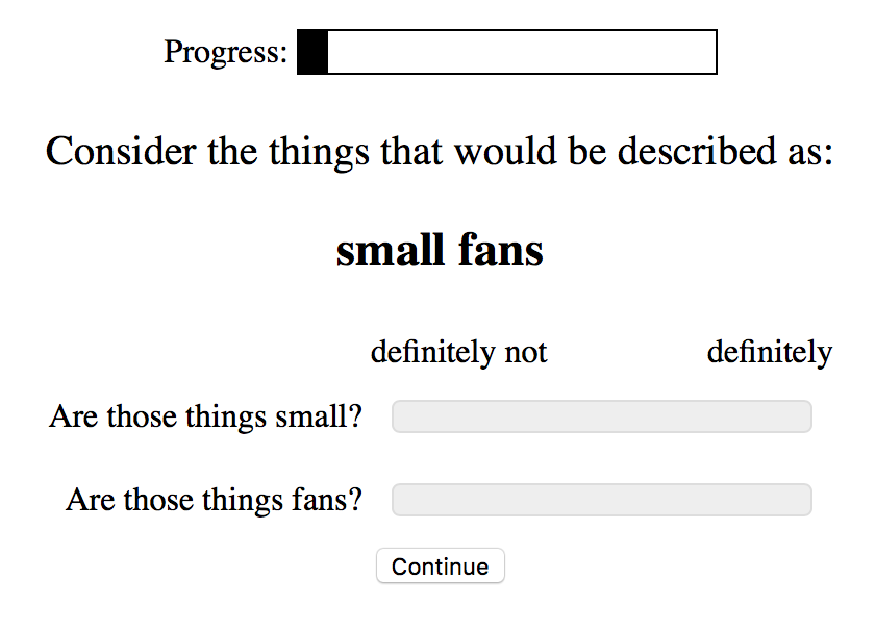
\includegraphics[width=3.75in]{images/concept_trial.eps}}
%	\caption{Example trial from the concept-formability experiment.}\label{concept-trial}
%\end{figure}
%
%\section{Results}
%
%We compared the concept formability ratings to the original naturalness ratings (Experiment 1). The adjective concept-formability ratings predict 8\% of the variance in our preference data (r$^{2}=0.08$; 95\% CI [0.00,  0.33]). The noun concept-formability ratings predict 36\% of the variance (r$^{2}=0.36$; 95\% CI [0.07,  0.62]). Recall that at its worst, subjectivity predicts 70\% of the variance in our preference data. 
%While it is quite possible that concept-formability plays an important role for some cases (such as \emph{arquitecte t\`{e}cnic}), we did not see evidence that it was critical to ordering preferences in our broad set of items. 
A theoretically neutral version of this compositional hypothesis is that some interaction between the noun and adjective will determine how closely the adjective is placed to the noun. This interaction could be caused by concept-formation, differential subjectivity, or other factors. We tested for such an interaction in our original naturalness ratings and found that noun-specific naturalness did not explain any variance in ordering preference above and beyond adjective-level naturalness. However, there were two adjective-noun pairs in our data with trends in the predicted direction: the naturalness ratings for \emph{hard} and \emph{soft} suggested a preference to occur closer to the noun \emph{cheese}. (Plausibly because hard and soft cheeses are complex concepts.) While these adjective-noun interactions do not survive correction for multiple comparisons in our statistical analysis, they do indicate that a different set of materials might---indeed, probably would---reveal by-noun effects on ordering preference. To follow up on this possibility, we re-ran our order preference and subjectivity experiments with a new set of materials that were chosen to maximize the probability of noun effects.


\section*{Experiment S1: Ordering preferences}

This experiment was a direct replication of our original naturalness ratings experiment (Experiment 1), using a different set of nouns. We chose nouns that we expected to form complex concepts and therefore yield effects on ordering preferences.

\paragraph{Participants.}

We recruited 50 participants through Amazon.com's Mechanical Turk crowd-sourcing service. Participants were compensated for their participation.

\paragraph{Design and methods.}

The design was identical to our original naturalness ratings experiment: participants were asked to indicate which of two object descriptions sounded more natural, using a sliding scale. Each description featured a noun modified by two adjectives; description pairs contained the same words with the relative adjective order reversed (e.g., ``the big blue thing'' vs.~``the blue big thing''). Adjectives were chosen at random from the original set of 26. The nouns were a reduced set of five (compared to the original ten). Nouns were chosen to maximize the probability of detecting noun-specific effects on adjective ordering preferences. In particular, we expected that nouns that are likely to form complex concepts should be 
%more likely to be involved in deviant adjective ordering preferences. Nouns that are likely to form complex concepts with an adjective are
highly collocational with that adjective. We thus searched for nouns that occur in particular adjective-noun phrases more frequently than predicted by the individual noun and adjective probabilities; in other words, nouns whose adjective-noun combinations were under-predicted by their individual word probabilities. %However, it was also important that the nouns exhibit a large range in under-predictedness (and consequently, in their collocational status). 

To find these nouns, we estimated the probability $p(A)$ of each adjective from our set of 26 by computing its relative frequency in an adjective-noun sequence in the BNC. We then computed the relative frequency of each noun $p(N)$ occurring in an adjective-noun sequence. Finally, we estimated the predicted joint probability of each adjective-noun combination by taking the product of each individual probability estimate: $\hat{p}(A,N) = p(A)\cdot p(N)$. Comparing  $\hat{p}(A,N)$ to the empirically estimated $p(A,N)$ establishes which adjective-noun combinations are under-predicted---more collocational---and thus likely to form complex concepts. We then restricted nouns to those 50 that maximize the observed range of under-predictedness while simultaneously requiring that each noun naturalistically occur with at least 11 of the 26 adjectives; from these 50 nouns, we selected the following four: \emph{apple, cheese, eyes, hair}. (Recall that \emph{cheese} occurred in our original materials, where it suggested possible by-noun effects with the adjectives \emph{hard} and \emph{soft}.) To these four nouns we added a fifth: \emph{thing}.
While \emph{thing} did not occur in the top 50, it did occur naturalistically with the most adjectives (23) out of the set of 26, thus allowing it to serve as a filler for the various object descriptions. The selected nouns, together with the number of adjectives they occur with, their range of ratios of empirical to predicted joint probabilities, and their minimum / maximum ratios, are shown in Table \ref{tab:nouns}.

\begin{table}
\centering
\begin{tabular}{l c c c c}
\toprule
Noun & \# of adjectives & range of ratios & minimum ratio & maximum ratio\\
\midrule
thing & 23 & 10.4 & 0.1 & 10.5 \\
eyes & 18 & 120.6 & 0.12 & 120.7 \\
hair & 15 & 82.9 & 0.03 & 83.0 \\
cheese & 13 & 114.0 & 0.4 & 114.4 \\
apple & 11 & 674.0 & 1.1 & 675.1 \\
\bottomrule
\end{tabular}
\caption{For each chosen noun, the number of adjectives (out of 26) that it occurs with; and for each adjective $A$ that the noun occurs with, the range of ratios $p(A,N) / \hat{p}(A,N)$ (empirical to predicted probability of occurrence); the minimum ratio; and the maximum ratio.}
\label{tab:nouns}
\end{table}




\paragraph{Results.}

To evaluate the role of specific noun information in determining ordering preferences, we performed the same nested linear model comparison from our original naturalness ratings experiment. The models we compared predicted naturalness ratings either by \textsc{adjective} (i.e., the adjective farthest from the noun) only, or by \textsc{adjective} together with its interaction with \textsc{noun} (i.e., the modified noun).
The model comparison revealed that noun-specific ratings did not explain any variance in ordering preference above and beyond adjective-level ratings ($F(1,225) = 0.93, p < 0.75$).  Thus, we again fail to find evidence of noun-specific effects on ordering preferences, this time in our new materials. 

\section*{Experiment S2: Subjectivity}

We next set out to replicate the finding that subjectivity predicts adjective ordering preferences in our new materials.

\paragraph{Participants.}

We recruited 40 participants through Amazon.com's Mechanical Turk crowd-sourcing service. Participants were compensated for their participation.

\paragraph{Design and methods.}

This experiment was a direct replication of our original faultless disagreement subjectivity experiment (Experiment 3), using the new set of nouns from the previous experiment.

\paragraph{Results.}

To evaluate the power of subjectivity in predicting adjective ordering preferences, we compared our new adjective subjectivity scores to the naturalness ratings collected in the previous experiment. 
Faultless disagreement scores account for  84\% of the variance in the new naturalness ratings ($r^2$ 0.84, 95\% CI [0.64,  0.91]; Fig.~S.1). 
%At the class level, faultless disagreement scores account for 86\% of the variance ($r^2$ = 0.86, 95\% CI [0.36, 0.99]).
%Given the greater ecological validity and better performance of our faultless disagreement measure, we  
As with our original materials, more subjective adjectives are preferred farther from the noun; subjectivity continues to predict adjective ordering preferences.


\renewcommand\thefigure{S.\arabic{figure}}
%\setcounter{figure}{}  
\begin{figure}
	\centering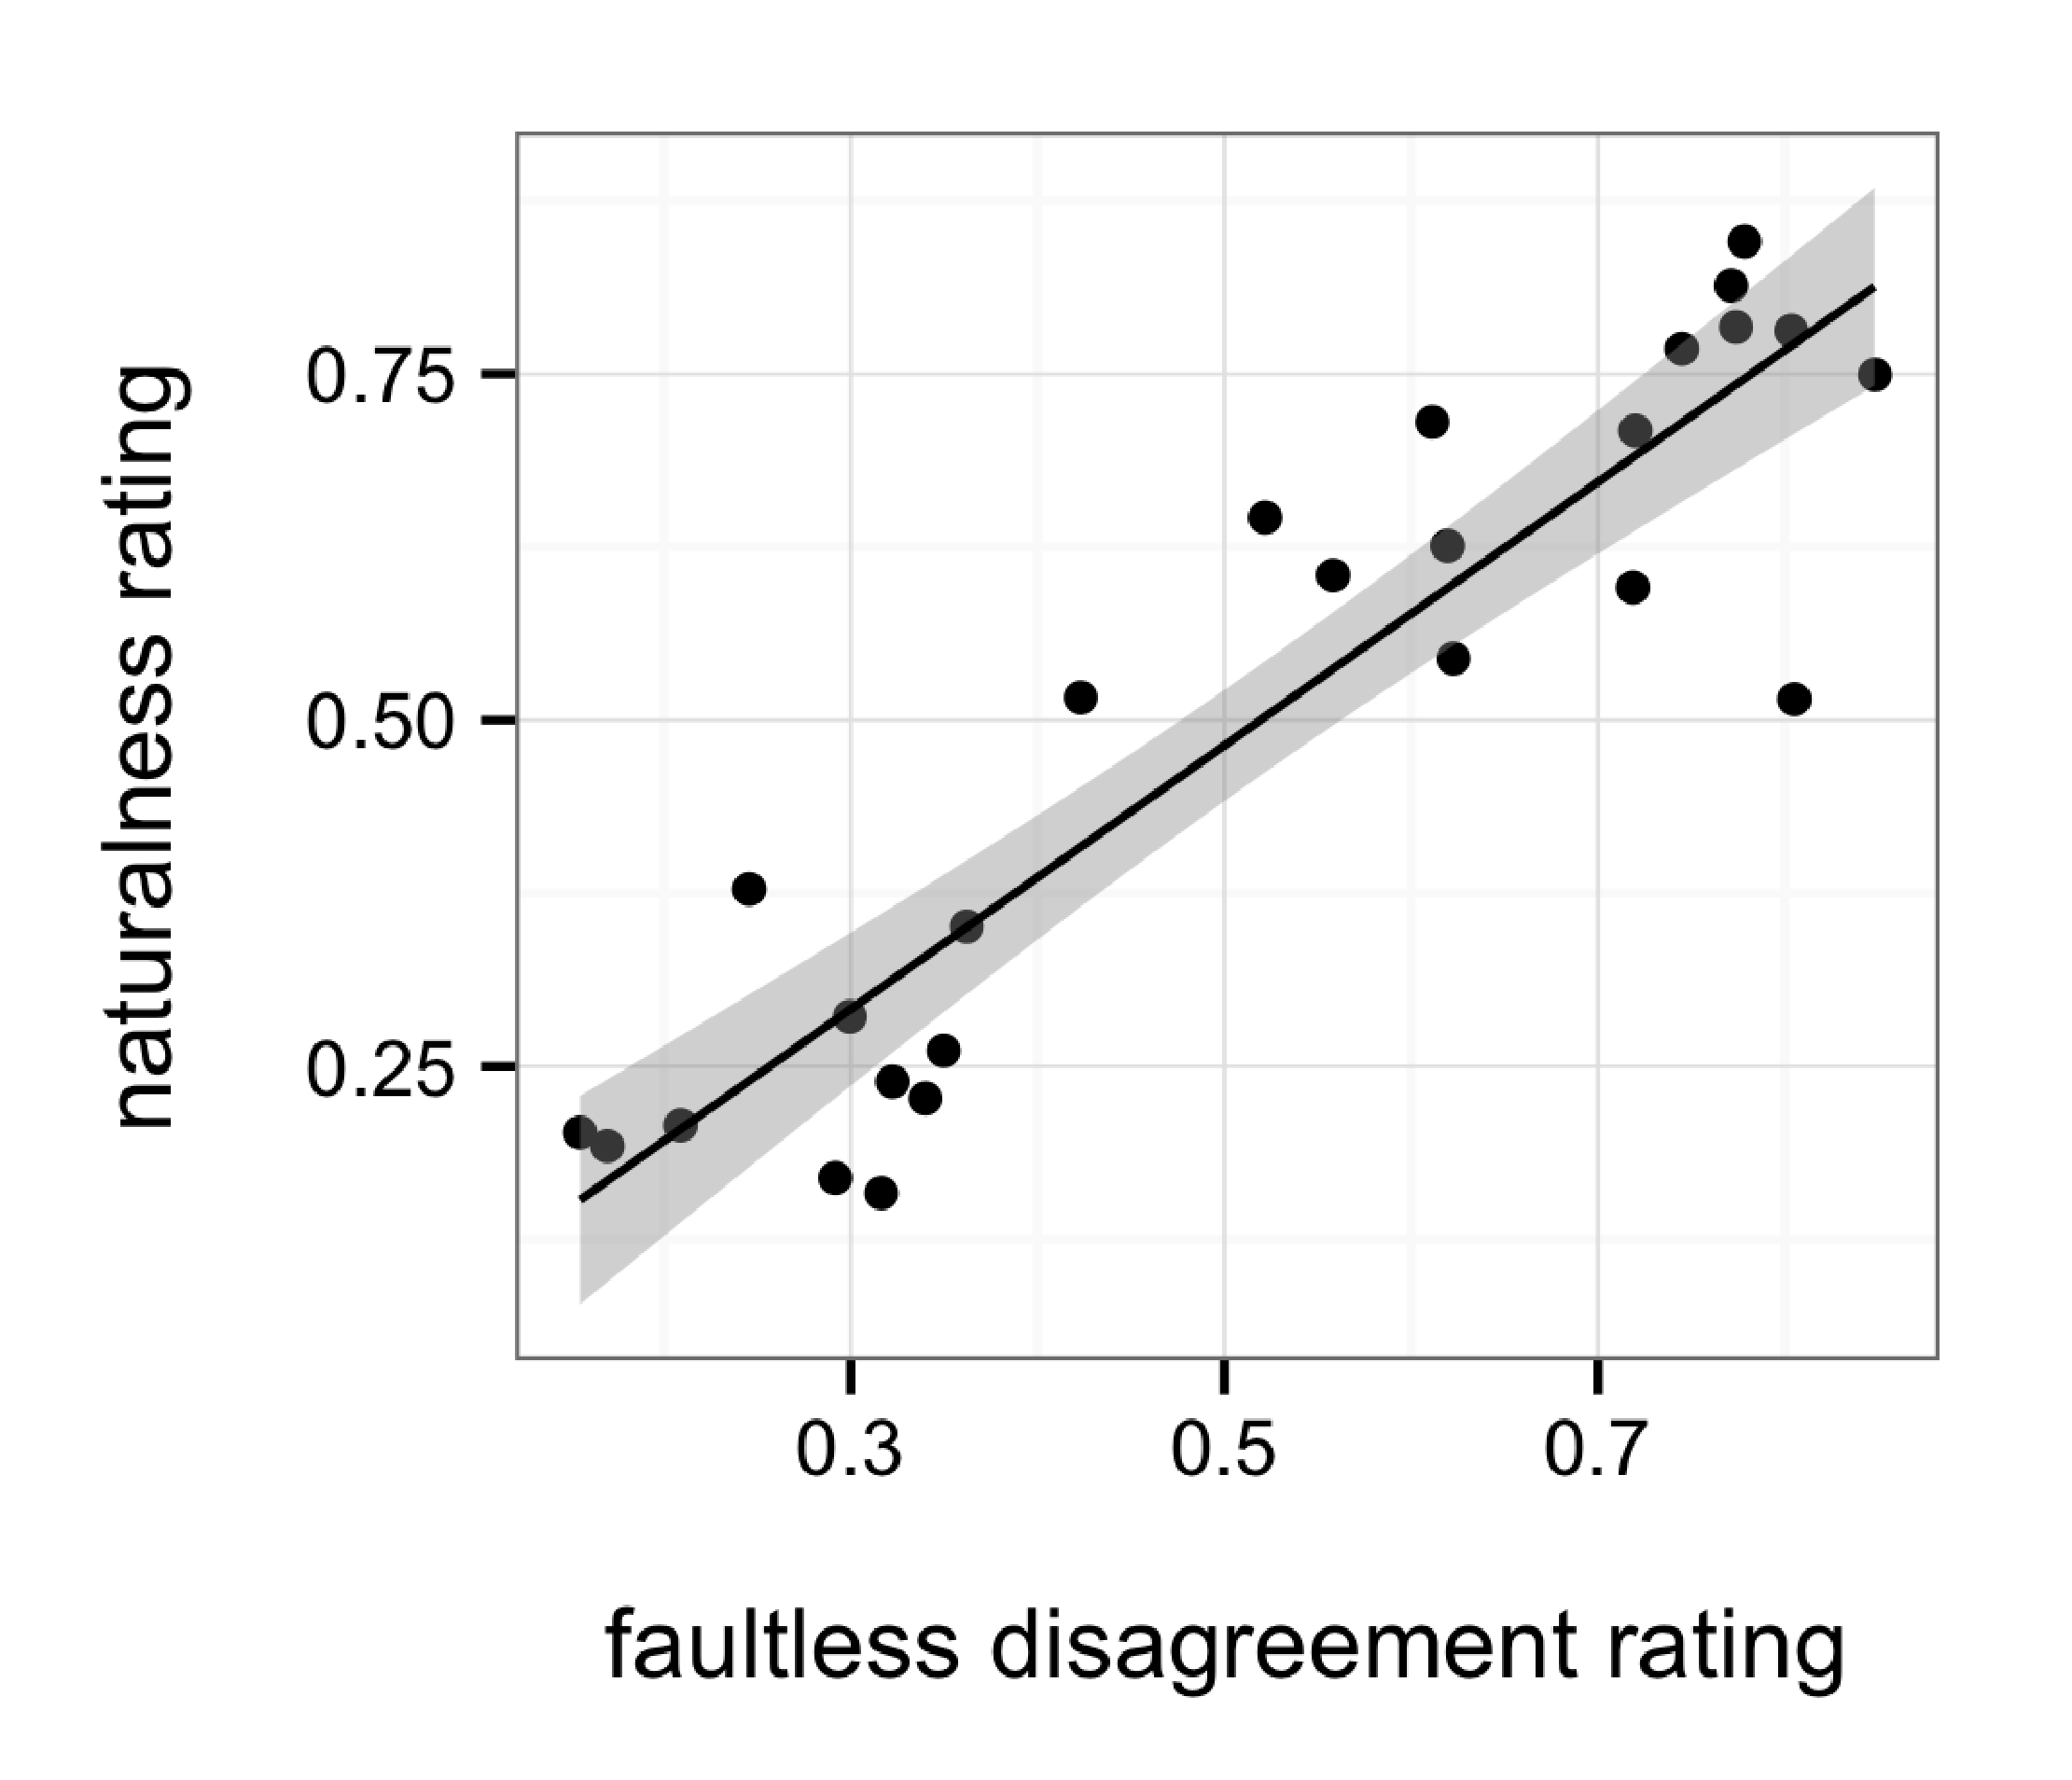
\includegraphics[width=2.8in]{plots/naturalness-faultless-new-nouns.eps}
	\caption{Mean naturalness ratings plotted against mean faultless disagreement scores for each of the 26 adjectives tested.}\label{naturalness-faultless-pred}
\end{figure}


\end{document}














